\chapter{Related Work}\label{sec:related-work}
There exists multiple of papers that provides a solution for SPH fluid surface extraction. The most popular trend  both in research community and in production is to extract surfaces from computed SDF on top of the Marching Cubes algorithm. One of the first methods proposed by Blinn uses the electron density function to compute an SDF. E.g. in \cite{Blinn} a sample function for a  hydrogen atom is:
\begin{equation}
	D(x) = e^{-a\cdot r(x)}
\end{equation}
where $r(x) = \sqrt{||x - x_1||_2}$ is a distance from the center of atom $x_1$ to point $x$. For the collection of atoms the function can be computed as:
\begin{equation}
	D(x) = \sum_j{b_j\cdot e^{-a\cdot r(x)}}
\end{equation}
Finally, a surface can be defined as those points where this density function equals some threshold amount ($T$):
\begin{equation}
	F(x) = D(x) - T
\end{equation}
However, the main disadvantage of such an SDF is that it is not able to generate flat surfaces, especially for particle sets with sharp features.\\

Müller et. al. in work \cite{Muller} proposed to use weighted density particle information for to extract SPH iso-surface. First smoothed color $cf_i$ is computed:
\begin{equation}
	cf_i = \sum_j{\dfrac{m_j}{\rho_j} \cdot W(x_i - x_j)}
\end{equation}
where $j$ are the neighboring particles of for $i$, $\rho_j$ is a density of a particle $j$, $m_j$ - mass and $W$ is a smoothing kernel function. The color field is 1 inside the fluid and 0 outside, the SDF can be defined as $F(x) = cf(x) - 0.5$, where $\sum_i cf_i * W(x - x_i)$.\\
Although the method performs better in terms of improving the quality of classical blobbies, it is still prone to generate small frequency bumps of the flat surface areas. This method produces relatively smooth surfaces, but in terms of removing significant amount of details (see figure \ref{fig:dam_break_comparison}).\\
Another method was developed by Zhu and Bridson (\cite{ZhuBridson}). The method constructs the SDF based only on the geometry information of the SPH particle set. The SDF is computed as 
\begin{equation}
	\phi(x) = |x - \bar{x}| - R
\end{equation}
where $\bar{x} = \sum_j{w_j \cdot x_j}$, R can be interpreted as a desired distance of the
surface from the particles, $x_j$ is a position of particle $j$, $r_j$ is a particle j's radii, $w_j$ is a weight of particle $j$, such that:
\begin{equation}
	w_j = \dfrac{W(|x - x_j|/R)}{\sum_i{W(x - x_i)/R}}
\end{equation}
The method reconstructs relatively smooth surface. However, the small frequency bumps still can be seen on the surface. Also the method has a known artifact near the concave regions due to nonuniform decay of the the weighted sum of neighbor SPH particle positions.\\
To solve the artifact introduced by Zhu \& Bridson method Solenthaler et. al. \cite{Solenthaler} proposed a solution using a distance decay function based on measuring the rate of change of the calculated center of  mass. The resulting SDF is calculated according to equation \ref{eq:solenthaler}
\begin{equation}
	\phi(x) = |x - \bar{x}| - Rf
	\label{eq:solenthaler}
\end{equation}
where f is calculated as:
\begin{equation}
	f = 
	\begin{cases}
		1 & \text{if $EVal_{max} < t_{min}$}\\
		\lambda^3 -3\cdot\lambda^2 + 3\lambda
	\end{cases}\\
\end{equation}
\begin{equation}
	\lambda = \dfrac{t_{max} - EVal_{max}}{t_{max} - t_{min}}
\end{equation}\\
Figure \ref{fig:ZB_vs_Solenthaler} shows some differences between ZhuBridson And Solenthaler methods.
\begin{figure}[H]
	\begin{center}
		\begin{subfigure}[b]{0.45\textwidth}
			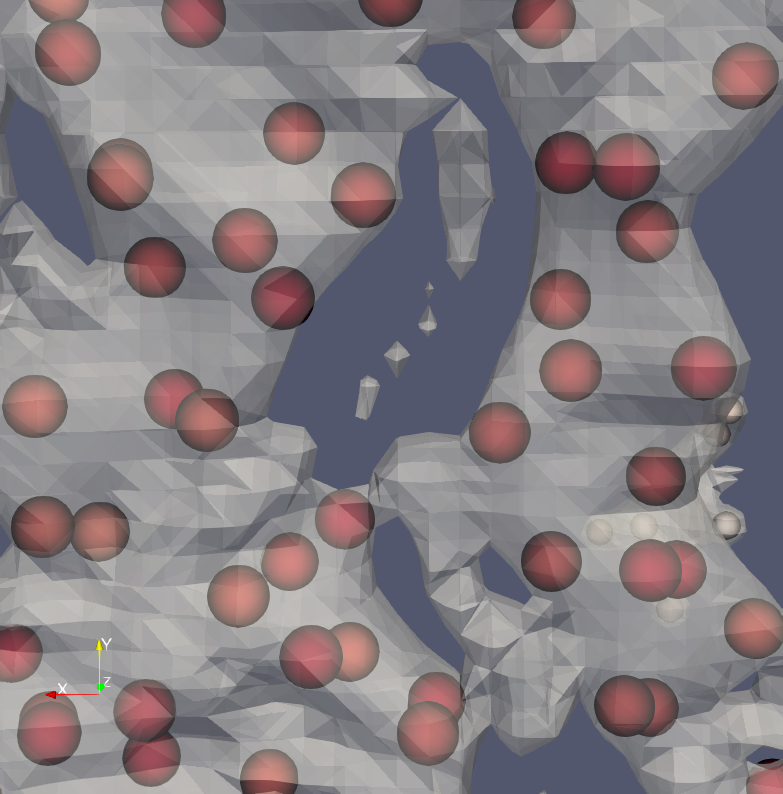
\includegraphics[width=\textwidth]{figures/GhostSurfaceZhuBridson.png}
		\end{subfigure}
		\begin{subfigure}[b]{0.45\textwidth}
			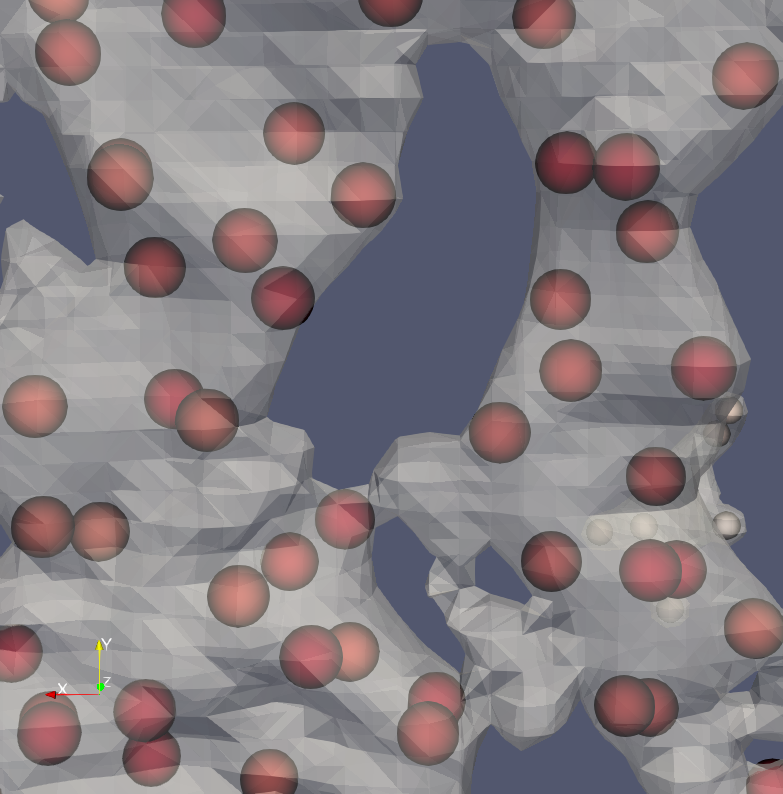
\includegraphics[width=\textwidth]{figures/GhostSurfaceSolenthaler.png}
		\end{subfigure}
	\end{center}
	\caption{Ghost surface artifact of ZhuBridson method (left), resolved by introducing the  distance decay function by Solenthaler et.al. (right)}
	\label{fig:ZB_vs_Solenthaler}
\end{figure}
Another attempt to improve surface quality was performed by J. Odenkirk et. al. in the work \cite{OnderikEtAl}. To make thin regions more compact so called density normalized method is applied. The SDF function now takes next shape:
\begin{equation}
	\phi(x) = |x - C(x)| - Rf(x)
\end{equation}
where :
\begin{equation}
	C(x) = \dfrac{\sum_j w_j^{-1} W(|x - x_j|, h) \cdot x_j}{\sum_j w_j^{-1} W(|x - x_j|, h)}
\end{equation}
$w_j$ is a normalization term, which can be computed as $w_j = \sum_i W(|x_j - x_i|, h)$. The distance decay
function is redefined:
\begin{equation}
	f(x) = g(w(x))
\end{equation}
where $g(w) = (1 - \dfrac{(w - w_{max})^2}{(w_{max} - w_{min})^2})^2$ and $w(x) = \sum_j{w_j^{-1} \cdot W(|x - x_j|, h)}$. However, the resulting surface looks rough (see Figure \ref{fig:dam_break_comparison}). Nevertheless, method computes the surface much faster than the Solenthaler method, which requires computing of covariance matrices and getting their eigenvalues for each MC grid vertex.\\
Some results of reconstructed scenes are presented in figures \ref{fig:dam_break_comparison}, \ref{fig:crown_comparison}, \ref{fig:double_dam_break_comparison} and \ref{fig:double_dam_break_comparison2}
\begin{figure}
	\begin{center}
		\begin{subfigure}[b]{0.48\textwidth}
			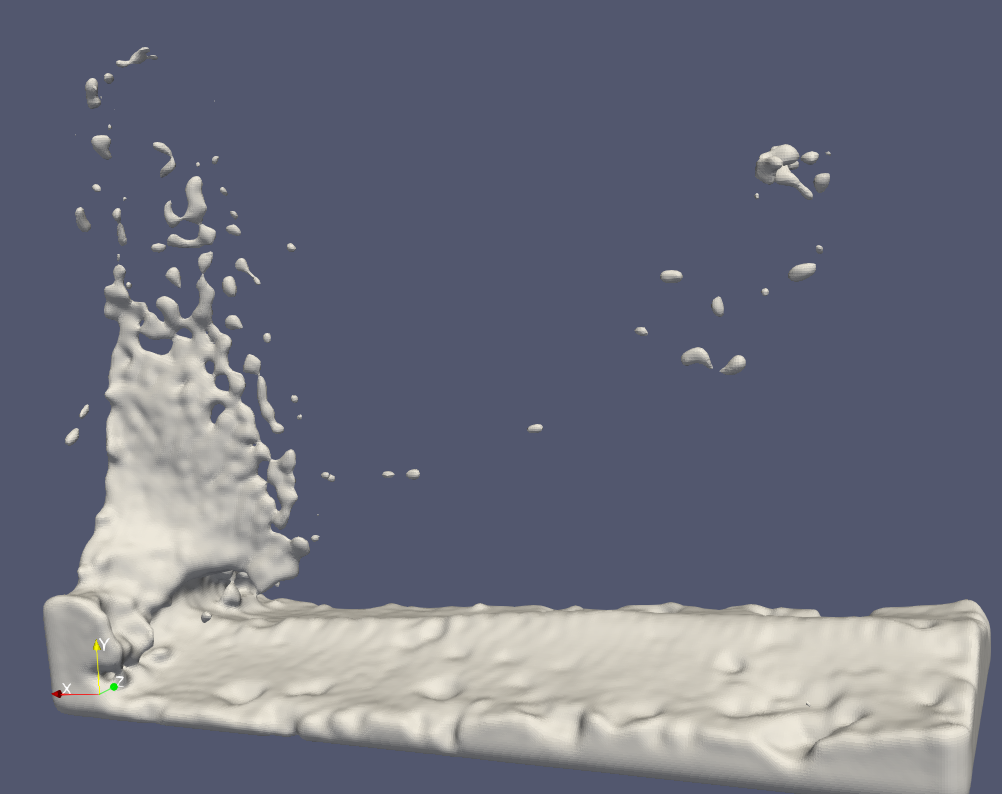
\includegraphics[width=\textwidth]{figures/MullerEtAlForRelWork.png}
			\caption{Muller et. al.}
		\end{subfigure}
		\begin{subfigure}[b]{0.48\textwidth}
			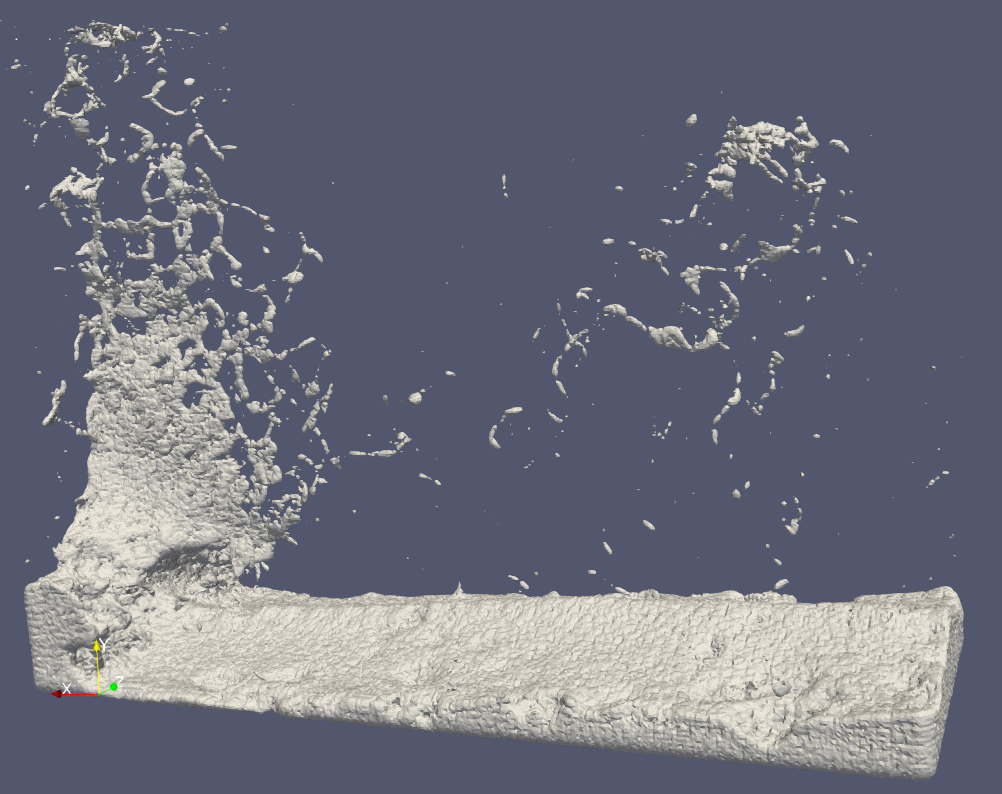
\includegraphics[width=\textwidth]{figures/OnderikEtAlForRelWork.png}
			\caption{Onderik et. al.}
		\end{subfigure}
		\begin{subfigure}[b]{0.48\textwidth}
			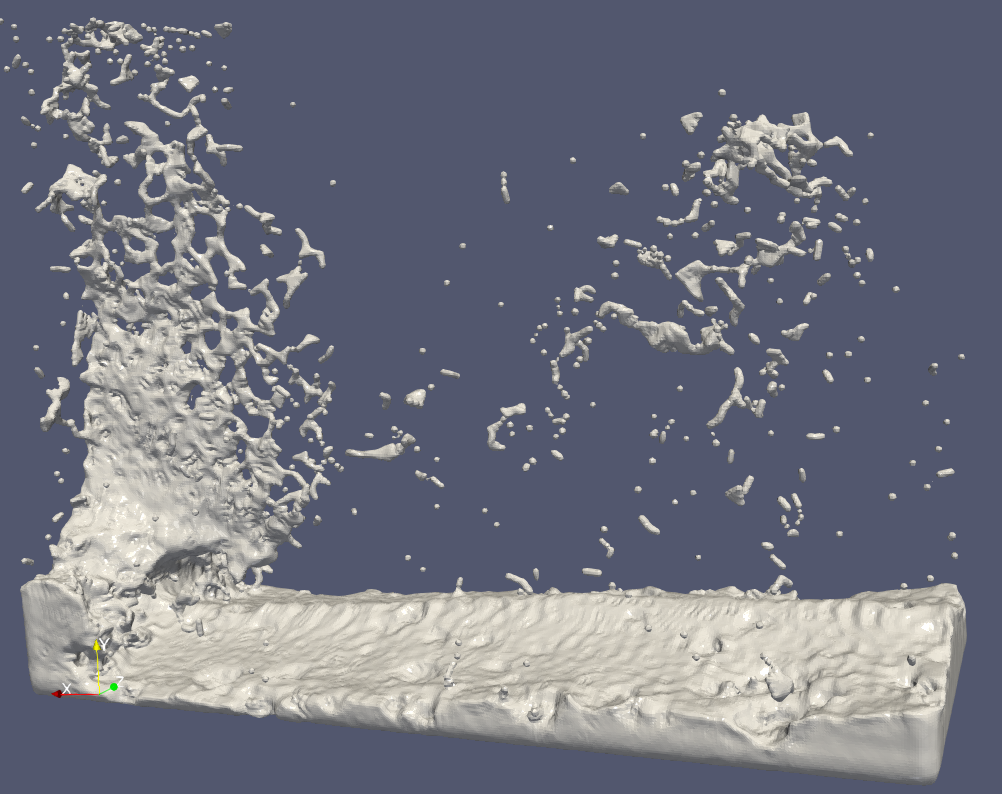
\includegraphics[width=\textwidth]{figures/SolenthalerEtAlForRelWork.png}
			\caption{Solenthaler et. al.}
		\end{subfigure}
		\begin{subfigure}[b]{0.48\textwidth}
			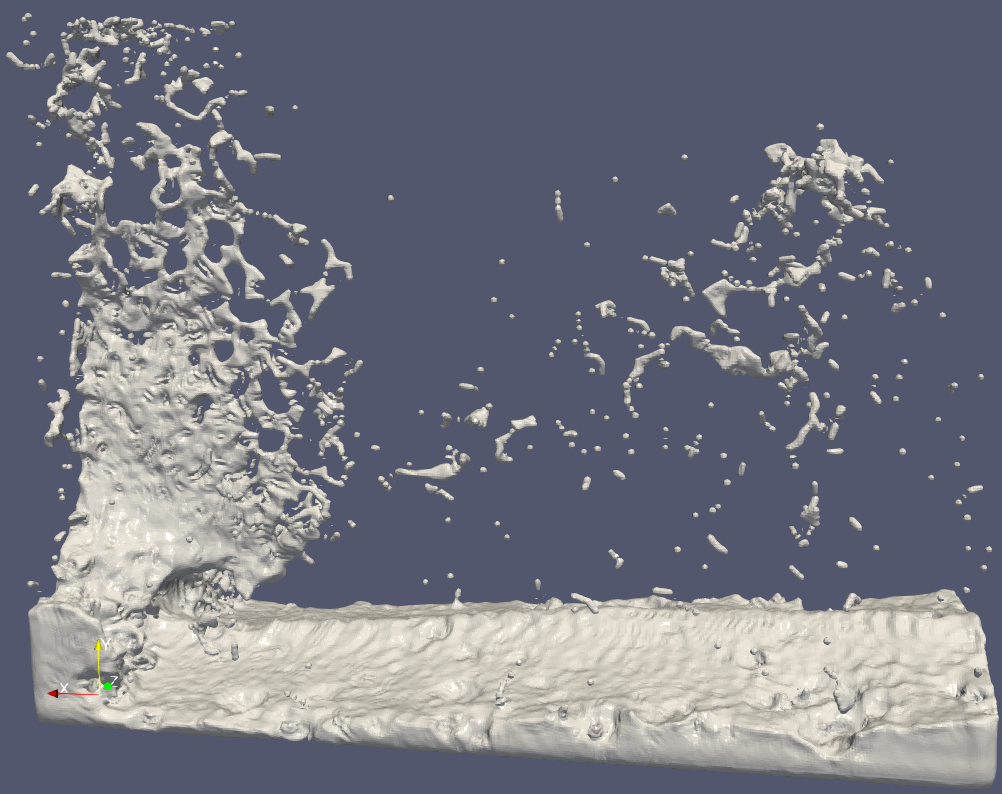
\includegraphics[width=\textwidth]{figures/ZhuBridsonForRelatedWorks.png}
			\caption{Zhu and Bridson}
		\end{subfigure}

	\end{center}
	\caption{Surface reconstruction methods comparison}
	\label{fig:dam_break_comparison}
\end{figure}
\begin{figure}
	\begin{center}
		\begin{subfigure}[b]{0.48\textwidth}
			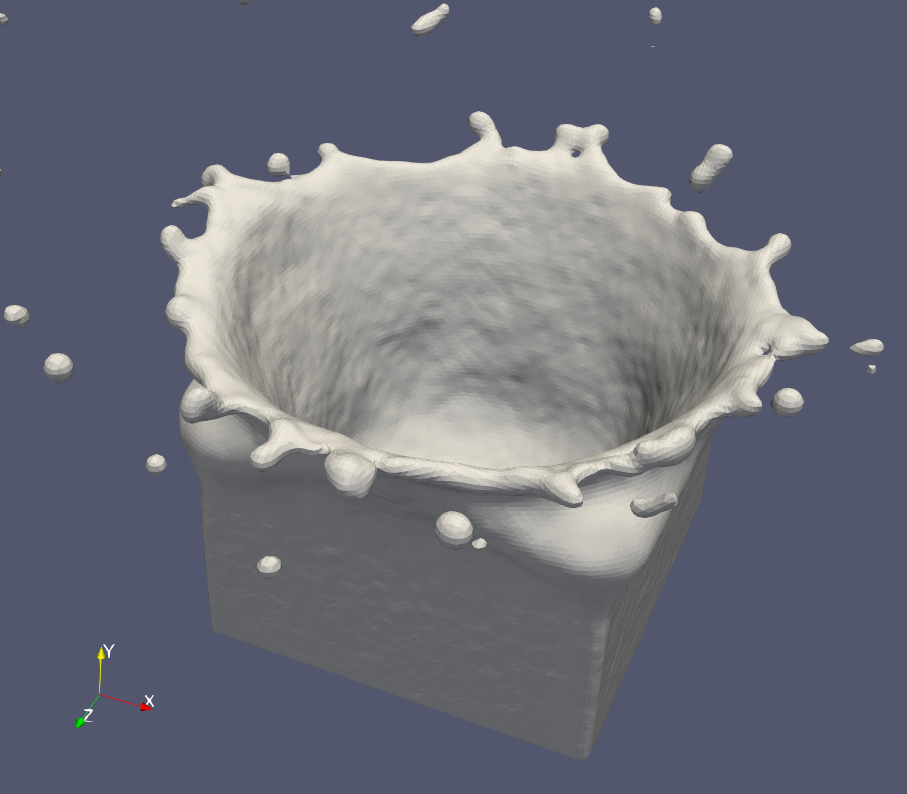
\includegraphics[width=\textwidth]{figures/MullerEtAlForRelWorkCrown.png}
			\caption{Muller et. al.}
		\end{subfigure}
		\begin{subfigure}[b]{0.48\textwidth}
			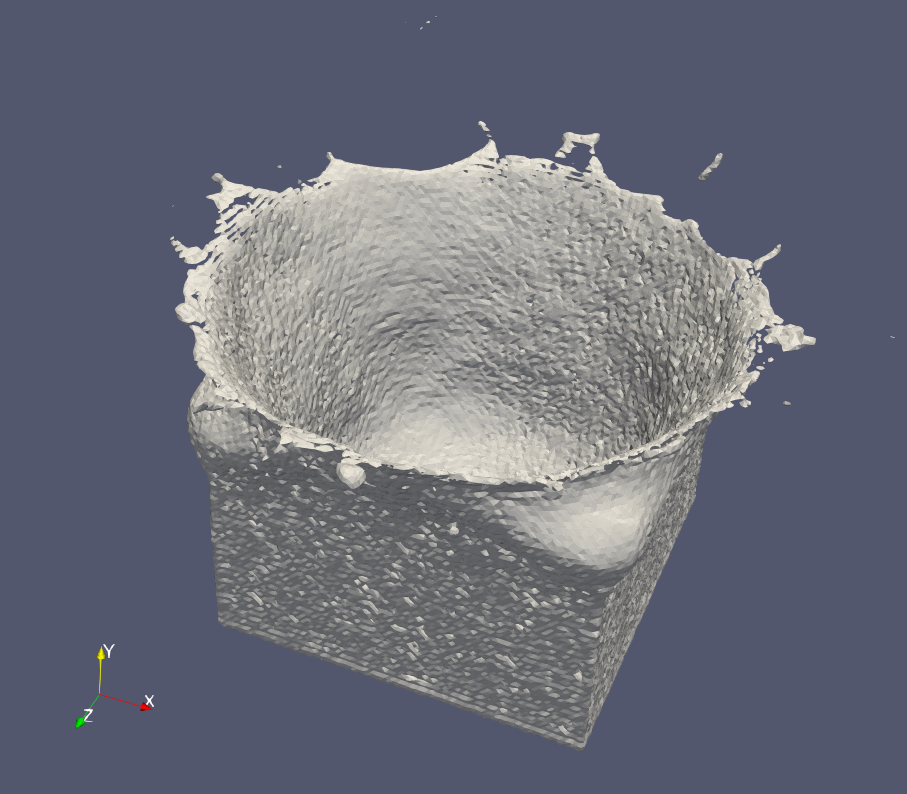
\includegraphics[width=\textwidth]{figures/OnderikEtAlForRelWorkCrown.png}
			\caption{Onderik et. al.}
		\end{subfigure}
		\begin{subfigure}[b]{0.48\textwidth}
			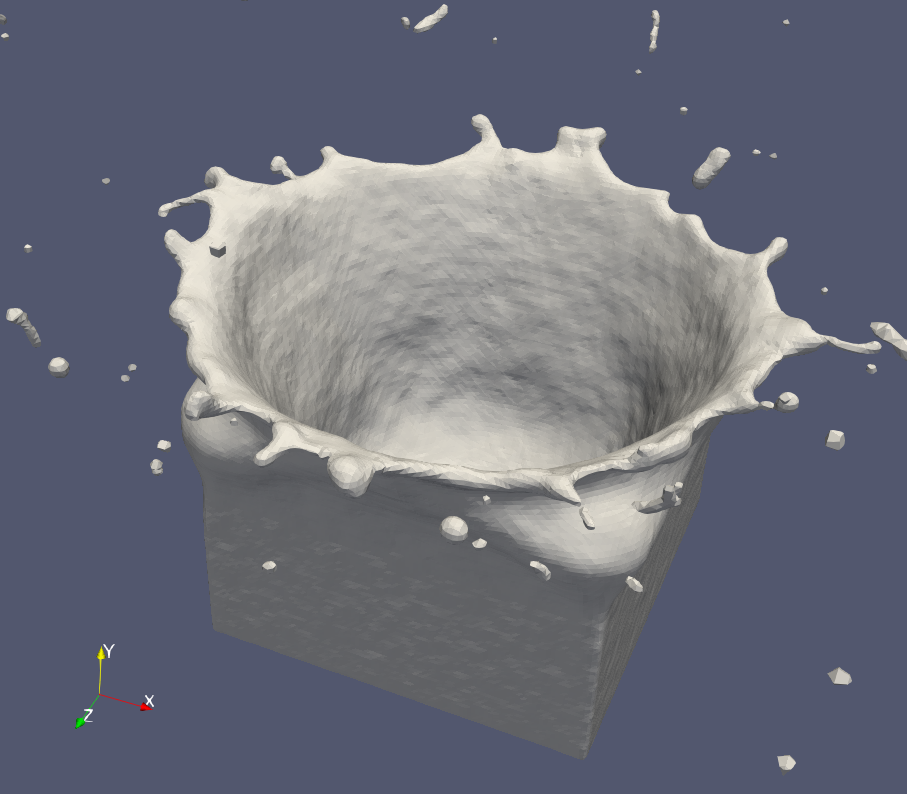
\includegraphics[width=\textwidth]{figures/SolenthalerEtAlForRelWorkCrown.png}
			\caption{Solenthaler et. al.}
		\end{subfigure}
		\begin{subfigure}[b]{0.48\textwidth}
			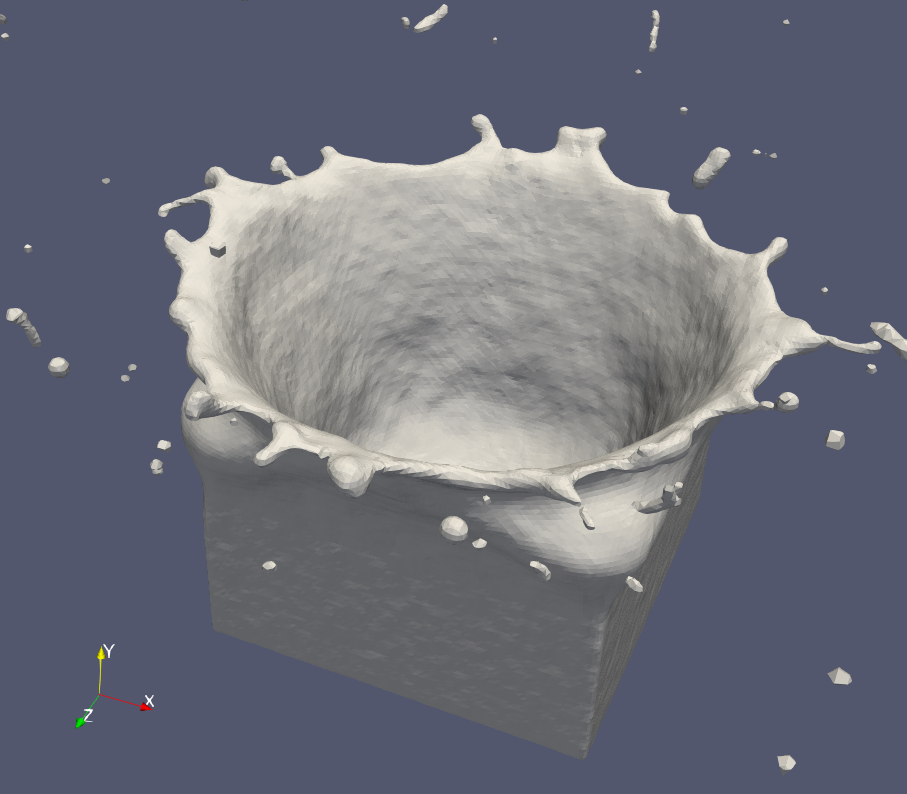
\includegraphics[width=\textwidth]{figures/ZhuBridsonForRelatedWorksCrown.png}
			\caption{Zhu and Bridson}
		\end{subfigure}

	\end{center}
	\caption{Surface reconstruction methods comparison of fluid crown after the splash}
	\label{fig:crown_comparison}
\end{figure}
\begin{figure}
	\begin{center}
		\begin{subfigure}[b]{0.48\textwidth}
			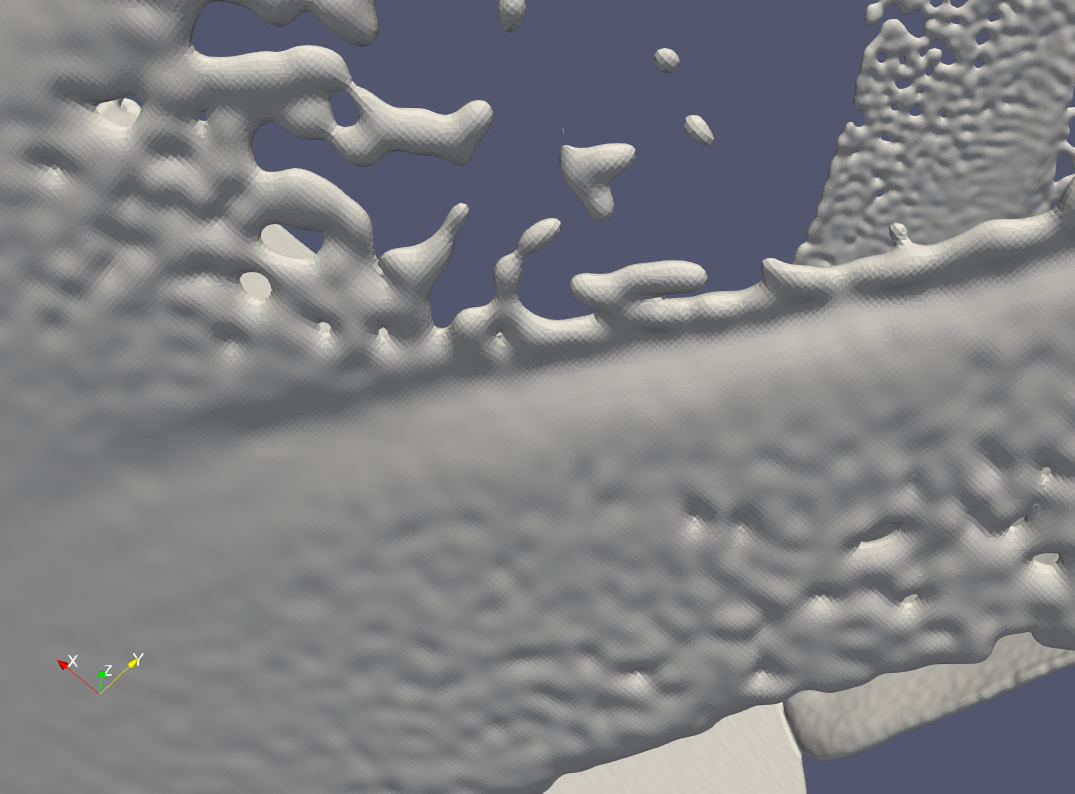
\includegraphics[width=\textwidth]{figures/MullerEtAlForRelWorkDoubleDamBreak.png}
			\caption{Muller et. al.}
		\end{subfigure}
		\begin{subfigure}[b]{0.48\textwidth}
			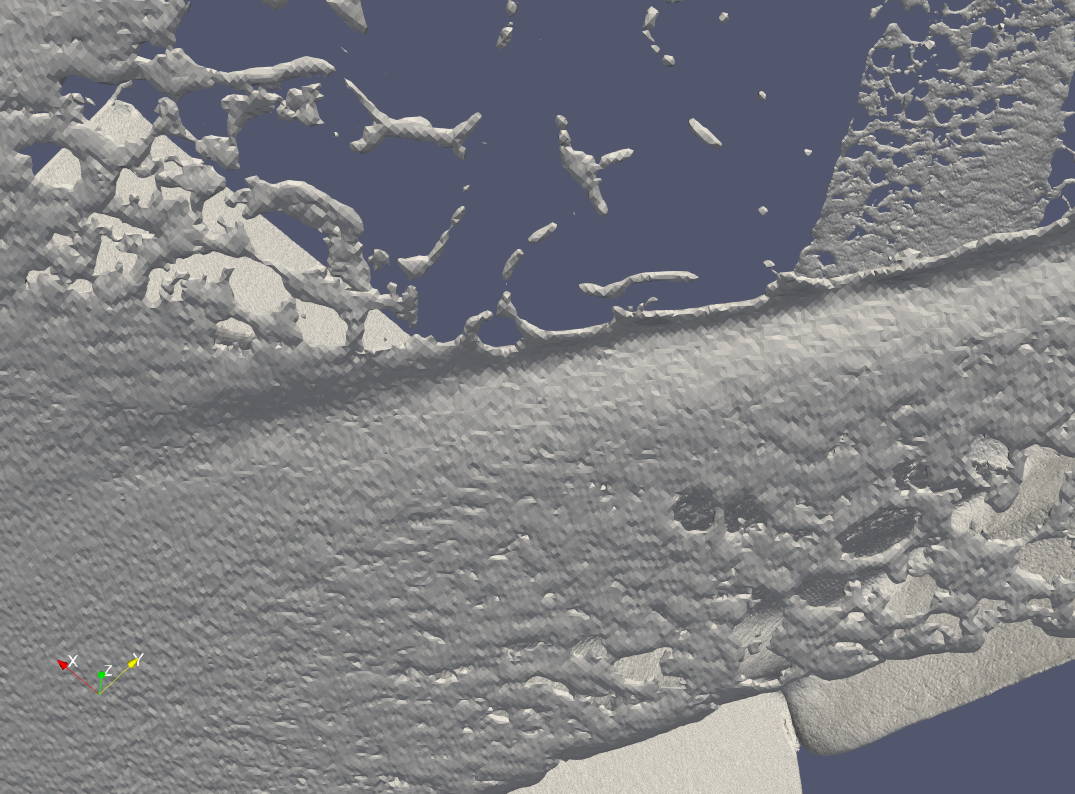
\includegraphics[width=\textwidth]{figures/OnderikEtAlForRelWorkDoubleDamBreak.png}
			\caption{Onderik et. al.}
		\end{subfigure}
		\begin{subfigure}[b]{0.48\textwidth}
			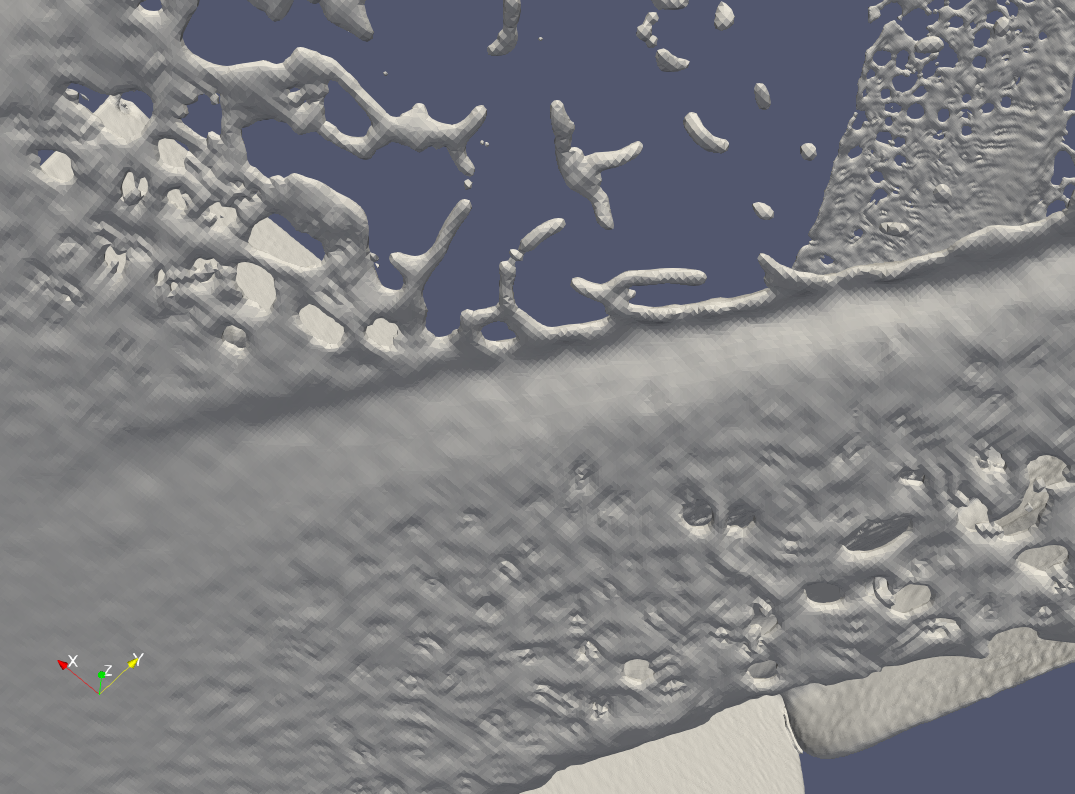
\includegraphics[width=\textwidth]{figures/SolenthalerEtAlForRelWorkDoubleDamBreak.png}
			\caption{Solenthaler et. al.}
		\end{subfigure}
		\begin{subfigure}[b]{0.48\textwidth}
			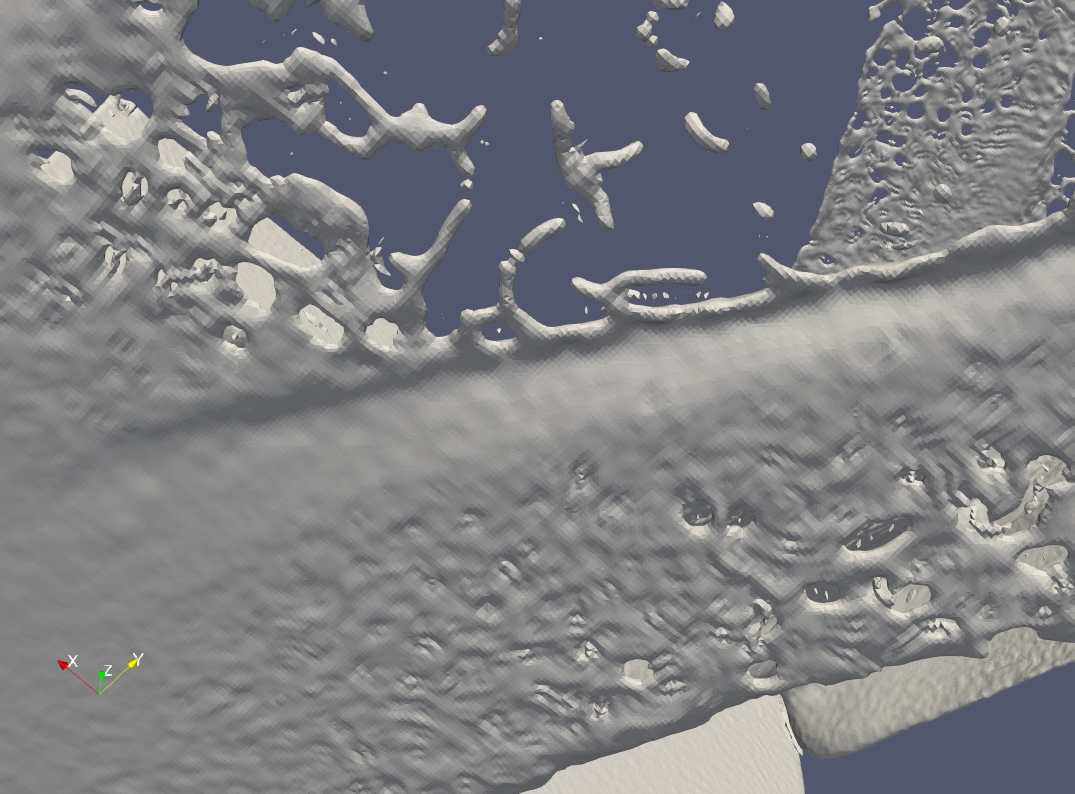
\includegraphics[width=\textwidth]{figures/ZhuBridsonForRelatedWorksDoubleDamBreak.png}
			\caption{Zhu and Bridson}
		\end{subfigure}

	\end{center}
	\caption{Surface reconstruction methods comparison of double dam break scenario}
	\label{fig:double_dam_break_comparison}
\end{figure}
\begin{figure}
	\begin{center}
		\begin{subfigure}[b]{0.48\textwidth}
			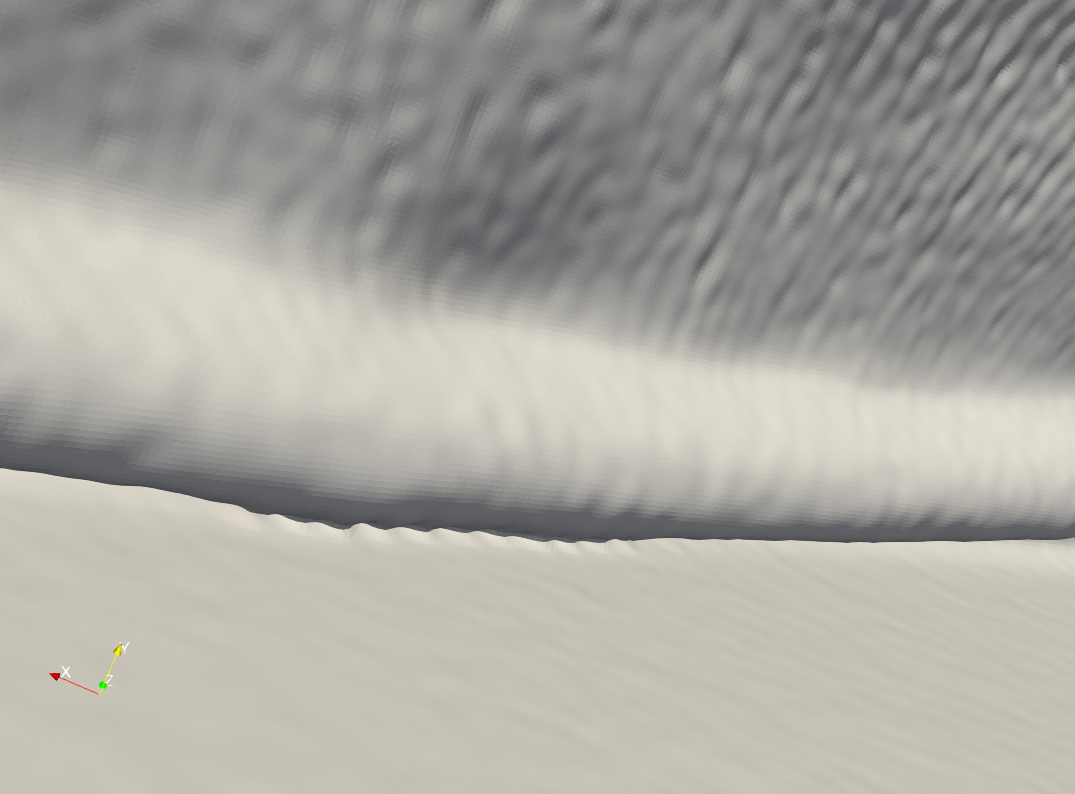
\includegraphics[width=\textwidth]{figures/MullerEtAlForRelWorkDoubleDamBreak2.png}
			\caption{Muller et. al.}
		\end{subfigure}
		\begin{subfigure}[b]{0.48\textwidth}
			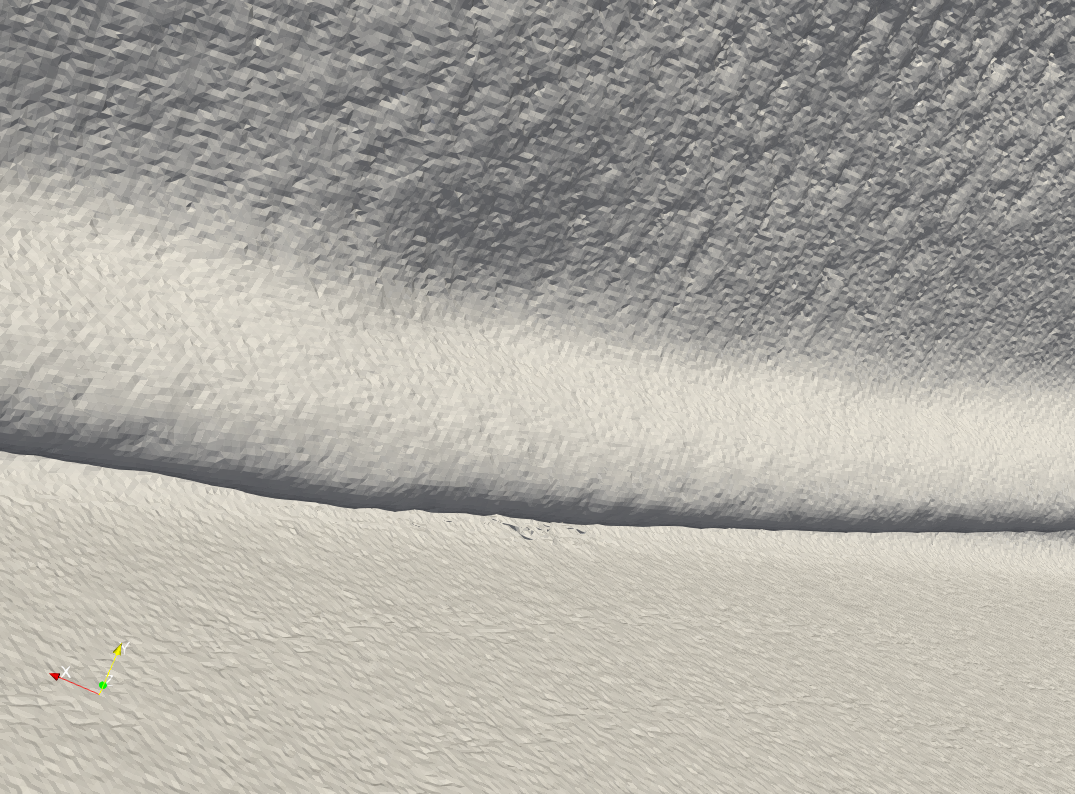
\includegraphics[width=\textwidth]{figures/OnderikEtAlForRelWorkDoubleDamBreak2.png}
			\caption{Onderik et. al.}
		\end{subfigure}
		\begin{subfigure}[b]{0.48\textwidth}
			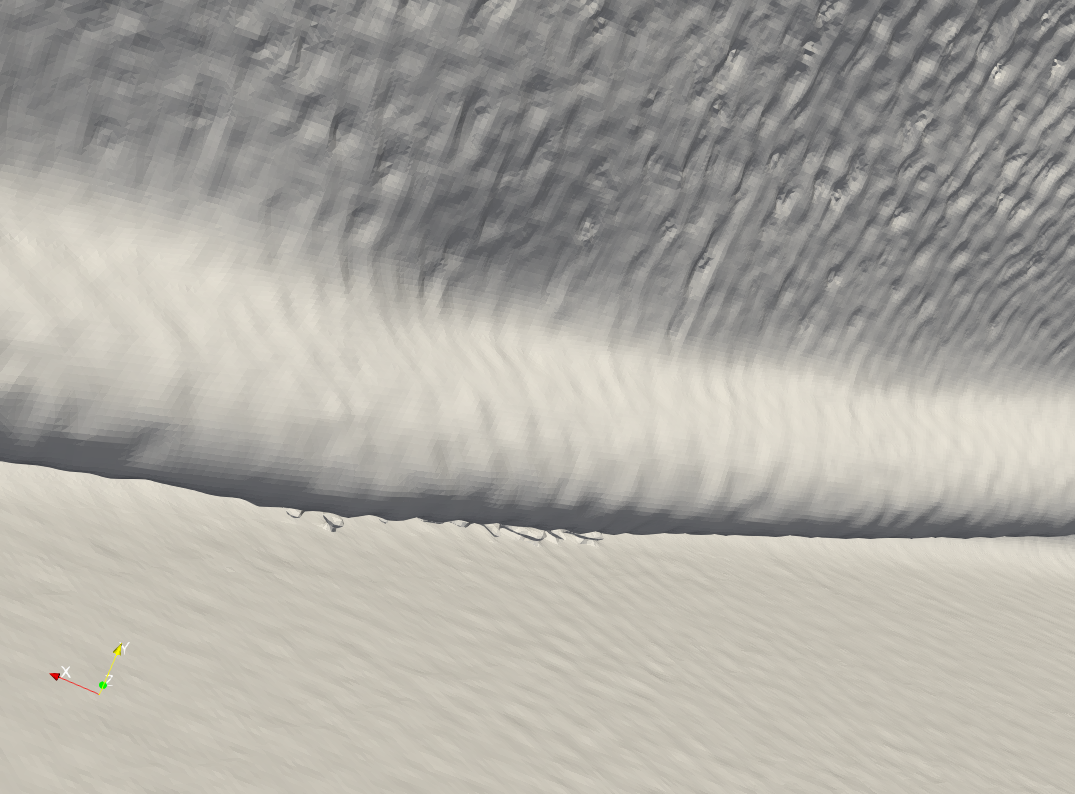
\includegraphics[width=\textwidth]{figures/SolenthalerEtAlForRelWorkDoubleDamBreak2.png}
			\caption{Solenthaler et. al.}
		\end{subfigure}
		\begin{subfigure}[b]{0.48\textwidth}
			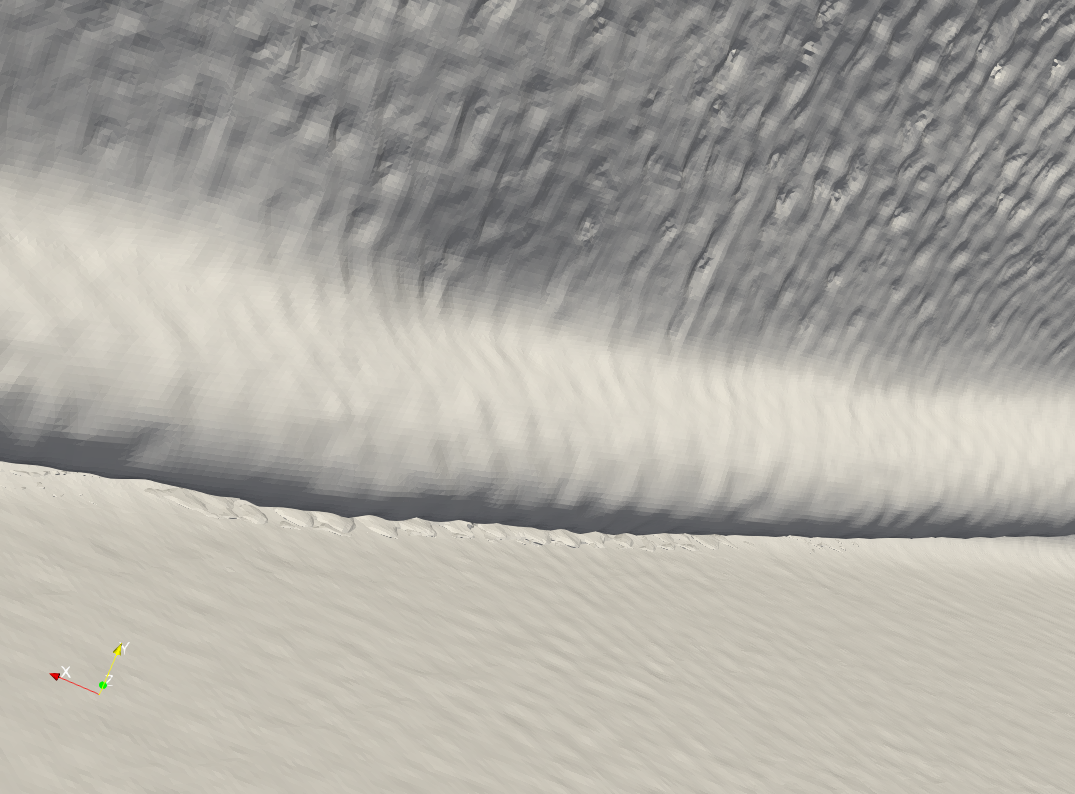
\includegraphics[width=\textwidth]{figures/ZhuBridsonForRelatedWorksDoubleDamBreak2.png}
			\caption{Zhu and Bridson}
		\end{subfigure}

	\end{center}
	\caption{Surface reconstruction methods comparison of double dam break scenario}
	\label{fig:double_dam_break_comparison2}
\end{figure}



Table \ref{tab:reconstruction_time} shows the reconstruction time for each method.
\begin{table}[h]
	\begin{center}
		\scriptsize
		\begin{tabular}{|l|c|c|c|c|c|c|}
			\hline
			Simulation type & Muller et.al. & Zhu \& Bridson & Solenthaler & Onderik et.al. \\
			\hline
			Reconstruction time		&	6.546929	&	4.329435	&	12.281569	&	4.232144	\\
			\hline
		\end{tabular}
	\end{center}
	\caption{Performance comparison for different reconstruction methods in seconds}
	\label{tab:reconstruction_time}
\end{table}

Adams et.al int the work \cite{AdamsEtAl} proposed SDF which is similar to Zhu Bridson's formulation: their definition can be obtained for Zhu \& Bridson by particle radii by particle–to–surface distances $d_i$. The SDF is defined as the following level set function:
\begin{equation}
	\phi(x) = d(x) - |x - \bar(x)|
\end{equation}
with
\begin{equation}
	d(x) = \sum_i W(|x - x_i|,h)\cdot d_i
\end{equation}
where $d_i$ is a approximate particle–to–surface distances. This re-distancing can be implemented by projecting particles near the surface onto the surface and propagating the distance information to the other particles in the interior of the fluid volume. The definition approximates flat surfaces as well as curve areas very well, however re-distancing requires additional computation effort w.r.t. to other methods.\\
One of the most promising methods, which produces smooth surfaces for flat and curve areas was proposed by Yu. and Turk. in the work \cite{YuTurk}. Their idea was to use anisotropic kernels instead of generally used isotropic used in \cite{Muller}. Anisotropic kernels are calculated as:
\begin{equation}
	W(|x_i - x_j|, G) = \tau \cdot  ||G|| \cdot P(||G \cdot (x_i - x_j)||)
\end{equation}
where G is linear transformation G rotates and stretches the radial vector $x_i - x_j$ depending on the neighborhood particles displacement, and P is a Gaussian function such as cubic spline. The method reconstructs very smooth surface, but requires computation of matrix $G$ for each SPH particle, thus extending reconstruction time significantly. Figure \ref{fig:Adams_vs_YoTurk} shows the difference between the results of the simulation for the Adams et.al. and Yu et.al. reconstruction techniques.
\begin{figure}[H]
	\begin{center}
		\begin{subfigure}[b]{0.48\textwidth}
			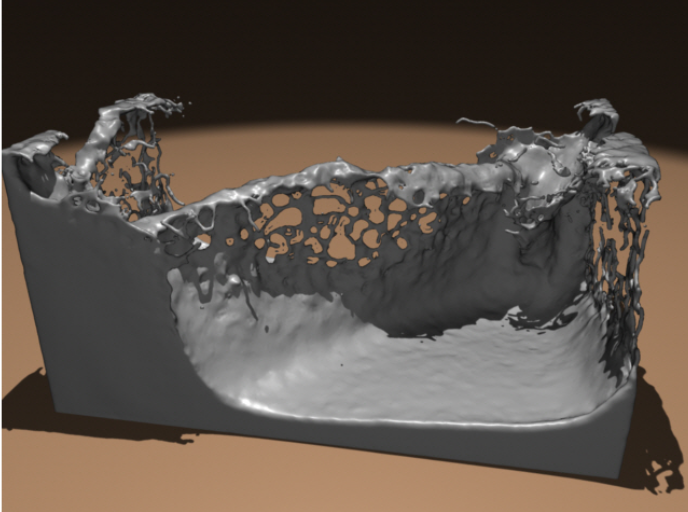
\includegraphics[width=\textwidth]{figures/Adams.et.al.Reconstruction.png}
			\caption{Adams et.al.}
		\end{subfigure}
		\begin{subfigure}[b]{0.48\textwidth}
			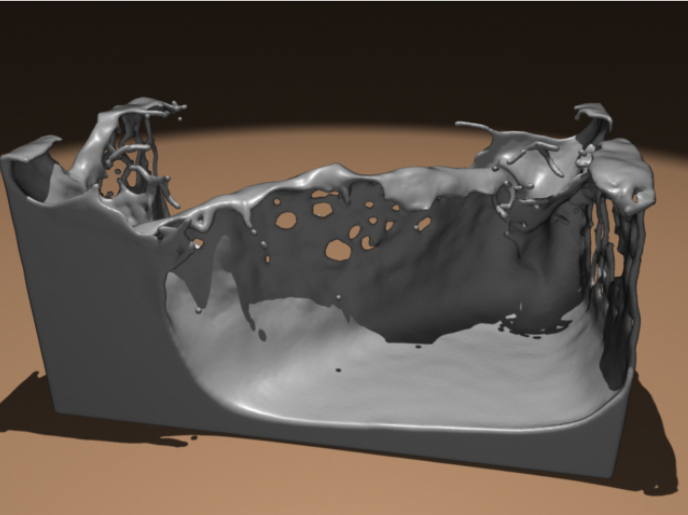
\includegraphics[width=\textwidth]{figures/Ya_and_Turl.Reconstruction.png}
			\caption{Yu and Turk}
		\end{subfigure}
	\end{center}
	\caption{Comparison between different surface reconstruction approaches on the Double dam break animation \cite{YuTurk}.}
	\label{fig:Adams_vs_YoTurk}
\end{figure}
The anisotropic kernel method leads to the realistic visualization of fluid surfaces and outperforms existing methods for handling smooth and thin surfaces with sharp features. The simplicity and efficiency of our method facilitate the incorporation of our method with existing SPH simulation schemes with little additional effort.